% IE 643 course project poster (novelty assessment), A1 landscape (84.1 x 59.4 cm).
% Build (from this folder):   tectonic poster.tex
% Figures (from the repo root): python poster/scripts/make_plots.py
%                               python poster/scripts/make_example.py
%                               python poster/scripts/make_qr.py
% Every number is read from a file under results/; the source is in a comment next to it.
\documentclass[final]{beamer}
\usepackage[size=custom,width=84.1,height=59.4,scale=1.0]{beamerposter}
\usetheme{ie643}

\usepackage{graphicx}
\usepackage{booktabs}
\usepackage{tabularx}
\usepackage{array}
\usepackage{tikz}
\usetikzlibrary{positioning,arrows.meta,calc}

% A1 sizes (= 30/50/100 pt at A0 scaled by 0.71)
\renewcommand{\normalsize}{\fontsize{21.5}{27}\selectfont}
\renewcommand{\small}{\fontsize{19}{23.5}\selectfont}
\renewcommand{\footnotesize}{\fontsize{17}{21}\selectfont}
\renewcommand{\scriptsize}{\fontsize{14}{16.6}\selectfont}

\newlength{\sepwidth}\setlength{\sepwidth}{1.6cm}
\newlength{\colwidth}\setlength{\colwidth}{25.9cm}
\newcommand{\separatorcolumn}{\begin{column}{\sepwidth}\end{column}}
\newcommand{\captionof}[2]{\par\vskip0.3ex{\usebeamerfont{caption}\color{muted}\RaggedRight #2\par}}
\newcommand{\hl}[1]{{\color{accent}\textbf{#1}}}
\newcommand{\todo}[1]{{\color{red!70!black}\textbf{[TODO: #1]}}}
\newcolumntype{L}{>{\RaggedRight\arraybackslash}X}
\newlength{\qrunit}\newcommand{\qrmodules}{37}
\graphicspath{{figures/}}

\tikzset{
  box/.style={draw=ink, line width=0.9pt, inner sep=4pt, align=center, font=\footnotesize, text=ink},
  abox/.style={box, draw=accent, line width=1.6pt},
  arr/.style={-{Stealth[length=7pt]}, line width=1pt, draw=ink},
}

\begin{document}
\begin{frame}[t]
\vspace*{0.6cm}
\posterheader
  {
\includegraphics[height=5.0cm]{logo.png}}
  {IE 643 Course Project}
  {Cross-Template Key-Value Extraction from Scanned Forms}
  {Team Unemployed and Unsupervised}
  {Param Mehta (23b2439) \qquad Arjoe Basak (23b1295)}
  {23b2439@iitb.ac.in \qquad 23b1295@iitb.ac.in \qquad IIT Bombay}
  {
\includegraphics[height=4.6cm]{IE643-Logo.pdf}}

\vspace{0.6cm}
\begin{columns}[t]
\separatorcolumn
% ============================================================== COLUMN 1: problem, gap, contribution
\begin{column}{\colwidth}

\begin{block}{Abstract}
Form extractors trained on a few templates lose 21 F1 points on unseen templates. A zero-shot vision-language reader that must cite OCR lines beats a trained tagger there (\hl{76.5} vs 70.5 F1). The tagger wins again once it has seen 10 templates, and on tables. End-to-end key-value linking improves with layout geometry, not multilingual text.
\end{block}

\begin{block}{Introduction}
New vendors send forms in layouts no model has seen, and every new template otherwise means relabelling and retraining. We extract named fields with no document of the held-out template in training. Layout-aware transformers (LiLT, BROS, LayoutLMv3) encode each word with its box; vision-language models also read field names.\par
\textbf{Protocol.} VRDU registration forms, 200 training documents, 3 folds. MTL: all templates seen. UTL: one held out. Metric: exact-span entity F1.
\end{block}

\begin{block}{Starting point: the seen-unseen gap}
{\small
\begin{tabularx}{\linewidth}{@{}Lrrr@{}}
\toprule
Intensive phase, VRDU & MTL & UTL & Gap \\
\midrule
LiLT & 91.6 & 64.2 & 27.3 \\                          % results/master_architectural_benchmark.csv
Delaunay graph network & 86.0 & 42.1 & 43.9 \\        % same CSV
BROS, template-adversarial & 91.8 & 69.6 & 22.2 \\                             % results/vrdu_dann_bros/metrics.json
BROS Track-1 (windows, jitter) & \textbf{92.4} & \textbf{71.3} & \textbf{21.1} \\ % results/vrdu_track1_bros/metrics.json
\bottomrule
\end{tabularx}}
{\scriptsize\color{muted}BROS Track-1 UTL by fold: 83.4 / 72.1 / 58.4.\par}
\vspace{0.5ex}
Two fields cause most of the loss: foreign\_principle\_name (0--13 F1 for every model; each template words it differently) and Short-Form registrants (95\% of BROS's errors are the filer block).
\end{block}

\begin{block}{Novelty Assessment: New Approaches}
\begin{tikzpicture}
\node[draw=accent, line width=2.6pt, inner sep=12pt, text width=\linewidth-28pt, align=left] {%
\fontsize{27}{33.5}\selectfont
\begin{enumerate}\setlength{\itemsep}{0.6ex}
\item \textbf{Read, don't train, for unseen wording.} A grounded zero-shot reader scores \hl{76.5} vs \hl{70.5} for BROS on unseen templates\textsuperscript{\dag}; a per-field router scores \hl{79.2}.
\item \textbf{The advantage reverses.} BROS overtakes the reader at 10 seen FATURA templates and on line-item tables.
\item \textbf{Linking, measured end to end:} \hl{47.4} with LiLT, \hl{53.4} with BROS geometry (\hl{+5.9}); multilingual text costs 3.
\end{enumerate}};
\end{tikzpicture}

\vspace{0.9ex}
{\small
\begin{tabularx}{\linewidth}{@{}p{3.9cm}LL@{}}
\toprule
 & Prior / intensive phase & Ours \\
\midrule
Wording & trained tagger: 70.5 & cited-line reader: \textbf{76.5}; router \textbf{79.2} \\
Train/read & not measured & crossover at K = 5 templates \\
Link model & LiLT 47.4; multilingual 44.2 & BROS joint: \textbf{53.4} \\
Tables & not covered & DocILE row F1 \textbf{59.6} \\
\bottomrule
\end{tabularx}}
\end{block}

\end{column}
\separatorcolumn
% ============================================================== COLUMN 2: method, workflow, data, first result
\begin{column}{\colwidth}

\begin{block}{Methods and Approaches}
\centering
\begin{tikzpicture}[x=1cm,y=1cm]
\node[box, text width=8cm] (in) at (0,0) {page image + OCR words and boxes};
\node[box, text width=11.4cm] (bros) at (-6.25,-2.5) {\textbf{BROS-base encoder} (trained)\\384-word windows, overlap 128, soft vote};
\node[abox, text width=11.4cm] (vlm) at (6.25,-2.5) {\textbf{Qwen3-VL-8B, 4-bit} (zero-shot)\\OCR lines with ids + field descriptions};
\node[box, text width=3.3cm, minimum height=2.0cm] (bio) at (-10.15,-5.6) {BIO tagger\\fields};
\node[box, text width=3.3cm, minimum height=2.0cm] (bia) at (-6.25,-5.6) {biaffine linker\\key→value};
\node[box, text width=3.3cm, minimum height=2.0cm] (row) at (-2.35,-5.6) {anchor rule\\cell→row};
\node[abox, text width=11.4cm, minimum height=2.0cm] (gr) at (6.25,-5.6) {JSON \{field: copied text, line id\}\\grounded back to OCR words};
\node[abox, text width=11cm] (rt) at (0,-8.4) {\textbf{per-field router}: BROS or reader};
\draw[arr] (in.south) -- ++(0,-0.5) -| (bros.north);
\draw[arr] (in.south) -- ++(0,-0.5) -| (vlm.north);
\foreach \n in {bio,bia,row} \draw[arr] (bros.south -| \n.north) -- (\n.north);
\draw[arr] (vlm) -- (gr);
\draw[arr] (bio.south) |- (rt.west);
\draw[arr] (gr.south) |- (rt.east);
\end{tikzpicture}
\captionof{figure}{One tagger, three light heads: a key→value pair and a table row are both links between detected cells.}
\end{block}

\begin{block}{Workflow}
\centering
\begin{tikzpicture}[node distance=0.4cm and 0.6cm,
  w/.style={box, text width=7.1cm, minimum height=2.0cm}, wa/.style={w, draw=accent, line width=1.6pt}]
\node[w] (a) {\textbf{Intensive phase}\\LiLT, BROS, DANN, GNN};
\node[w, right=of a] (b) {\textbf{Error analysis}\\gap = 2 fields};
\node[wa, right=of b] (c) {\textbf{Zero-shot reader}\\+ router};
\node[wa, below=of c] (d) {\textbf{Grounded prompt}\\VRDU 76.5};
\node[wa, left=of d] (e) {\textbf{FATURA crossover}\\K = 1--40};
\node[wa, left=of e] (f) {\textbf{Linking end to end}\\47.4 → 53.4};
\node[wa, below=of f] (g) {\textbf{Link backbone}\\XLM, crops, BROS};
\node[wa, right=of g] (h) {\textbf{Tables}\\ad-buy, DocILE};
\node[w, right=of h] (i) {\textbf{Page pixels}\\LayoutLMv3};
\draw[arr] (a)--(b); \draw[arr] (b)--(c); \draw[arr] (c)--(d); \draw[arr] (d)--(e); \draw[arr] (e)--(f);
\draw[arr] (f)--(g); \draw[arr] (g)--(h); \draw[arr] (h)--(i);
\end{tikzpicture}
\captionof{figure}{Blue = novelty phase.}
\end{block}

\begin{block}{Dataset Details}
{\small
\begin{tabularx}{\linewidth}{@{}p{4.4cm}Lp{5.4cm}@{}}
\toprule
Dataset & Task and size & Unseen split \\
\midrule
VRDU forms & 6 fields; 1,915 docs, 3 templates & 1 held out \\
VRDU ad-buy & line items; 641 docs & N = 10--200 \\
FATURA & 9 fields; 50 templates × 200 & K = 1--40 seen \\
XFUND & links, 5 languages; 250 val forms & 94\% unseen \\
DocILE & 19 line-item fields; 5,680 docs & 200 new layouts \\
\bottomrule
\end{tabularx}}
\end{block}

\begin{block}{Results: unseen form templates}
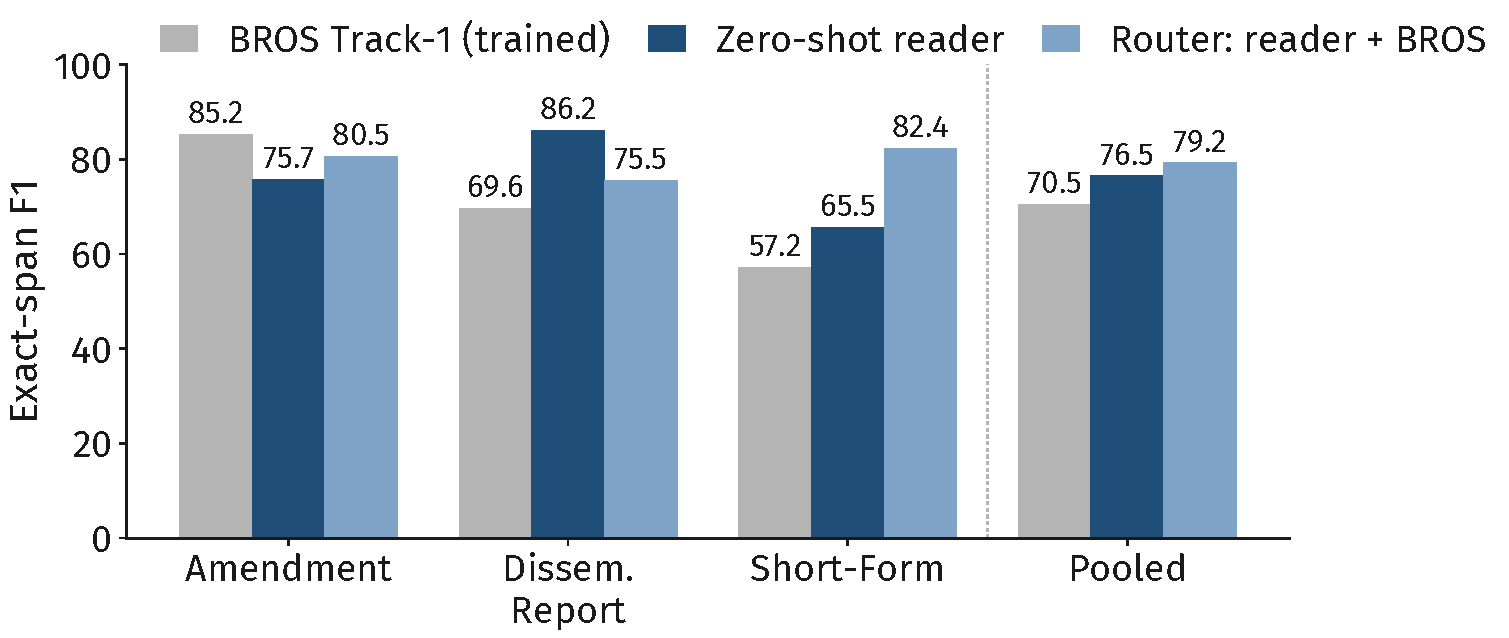
\includegraphics[width=0.84\linewidth]{f1_vrdu_templates.pdf}
\captionof{figure}{VRDU confirm set, 100 forms per template; BROS = mean of 2 seeds. Router +8.7 [+6.9, +10.6] pooled but −4.6 on Amendment. Dev set: 75.2 vs 69.8.}
\end{block}

\end{column}
\separatorcolumn
% ============================================================== COLUMN 3: results, conclusion, refs
\begin{column}{\colwidth}

\begin{block}{Results: when to train, when to read}
\begin{minipage}[t]{0.49\linewidth}
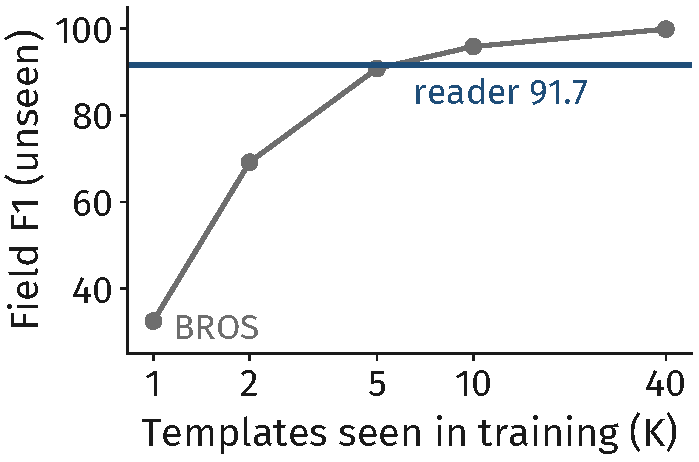
\includegraphics[width=\linewidth]{f2_fatura_crossover.pdf}
\captionof{figure}{FATURA. Tie at K = 5 (+0.9); BROS ahead by 4.2 at K = 10.}
\end{minipage}\hfill
\begin{minipage}[t]{0.49\linewidth}
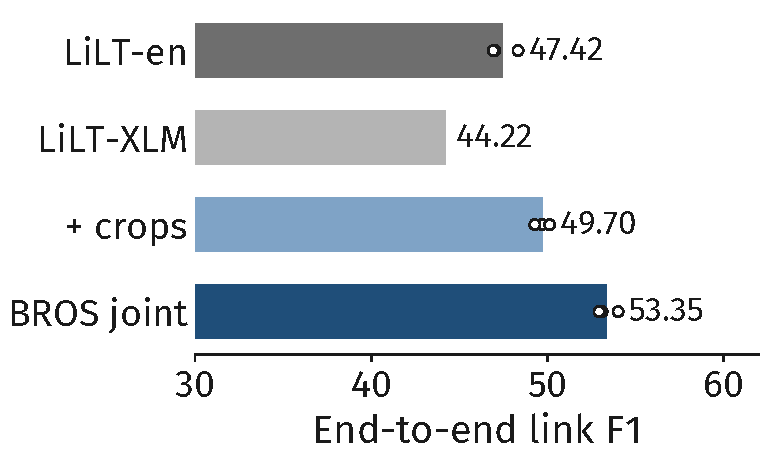
\includegraphics[width=\linewidth]{f3_xfund_links.pdf}
\captionof{figure}{XFUND link F1, end to end. LiLT-XLM is the multilingual encoder.}
\end{minipage}

\vspace{-0.4ex}
\begin{minipage}[t]{0.52\linewidth}
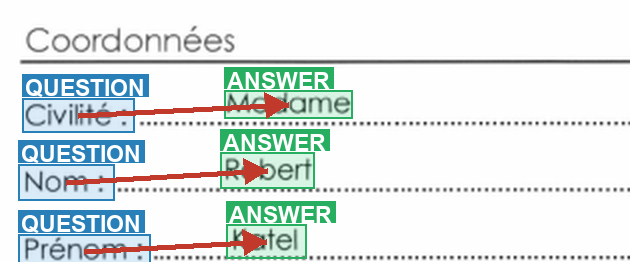
\includegraphics[width=\linewidth]{linking_fr.png}
\captionof{figure}{XFUND, unseen French form: our BROS model tags questions (blue) and answers (green) and links each question to its answer (red arrows).}
\end{minipage}\hfill
\begin{minipage}[t]{0.45\linewidth}
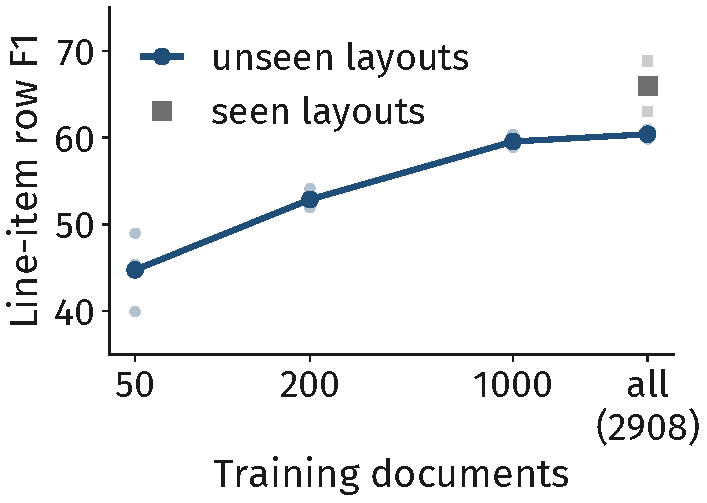
\includegraphics[width=0.9\linewidth]{f4_docile_curve.pdf}
\captionof{figure}{DocILE, BROS. Gap 2--9 points (VRDU: 21); 21.4\% of cells missed.}
\end{minipage}

\end{block}

\begin{block}{Conclusion and Future Work}
\begin{itemize}\setlength{\itemsep}{0.2ex}
\item Read when templates are new and few; train when 10+ are seen and for tables (ad-buy: reader 38.2 vs BROS 68.8--85.7 row F1).
\item Linking: geometry +5.9, multilingual text about −3. Pixels (LayoutLMv3 vs blank image): none on seen templates, +0.8 over three unseen (unstable seeds), 14 below BROS. Future work: a learned router.
\item Limits: \textsuperscript{\dag}prompt tuned on dev/confirm, fresh-form test not run.
\end{itemize}
\end{block}

\begin{block}{References}
\scriptsize\setlength{\parskip}{0.15ex}
Teakgyu Hong, Donghyun Kim, Mingi Ji, Wonseok Hwang, Daehyun Nam and Sungrae Park. BROS: A Pre-trained Language Model Focusing on Text and Layout for Better Key Information Extraction from Documents, AAAI, 2022. https://arxiv.org/abs/2108.04539\par
Jiapeng Wang, Lianwen Jin and Kai Ding. LiLT: A Simple yet Effective Language-Independent Layout Transformer for Structured Document Understanding, ACL, 2022. https://arxiv.org/abs/2202.13669\par
Yupan Huang, Tengchao Lv, Lei Cui, Yutong Lu and Furu Wei. LayoutLMv3: Pre-training for Document AI with Unified Text and Image Masking, ACM Multimedia, 2022. https://arxiv.org/abs/2204.08387\par
Zilong Wang, Yichao Zhou, Wei Wei, Chen-Yu Lee and Sandeep Tata. VRDU: A Benchmark for Visually-rich Document Understanding, KDD, 2023. https://arxiv.org/abs/2211.15421\par
Štěpán Šimsa, Milan Šulc, Michal Uřičář, et al. DocILE Benchmark for Document Information Localization and Extraction, ICDAR, 2023. https://arxiv.org/abs/2302.05658\par
Mahmoud Limam, Marwa Dhiaf and Yousri Kessentini. FATURA: A Multi-Layout Invoice Image Dataset for Document Analysis and Understanding, arXiv, 2023. https://arxiv.org/abs/2311.11856\par
Yiheng Xu, Tengchao Lv, Lei Cui, et al. XFUND: A Benchmark Dataset for Multilingual Visually Rich Form Understanding, Findings of ACL, 2022. https://aclanthology.org/2022.findings-acl.253\par
Qwen Team. https://huggingface.co/Qwen/Qwen3-VL-8B-Instruct, Accessed on: 22nd November, 2026.\par
\end{block}

\vspace{-0.8ex}
\begin{columns}[t,onlytextwidth]
\begin{column}{0.52\linewidth}
\begin{block}{Acknowledgements}
\small We thank the IE 643 instructor and TAs. GPU runs used Kaggle notebooks.
\end{block}
\end{column}
\begin{column}{0.22\linewidth}\centering{\footnotesize\textbf{GitHub}\par}\vspace{0.4ex}
\setlength{\qrunit}{3.5cm/\qrmodules}% https://github.com/ABasakEE/KeyValue-Extraction/tree/feat/bros-relative-layout
\begin{tikzpicture}[x=\qrunit,y=\qrunit]
\fill[ink] (0,36) rectangle ++(1,1) (1,36) rectangle ++(1,1) (2,36) rectangle ++(1,1) (3,36) rectangle ++(1,1) (4,36) rectangle ++(1,1) (5,36) rectangle ++(1,1) (6,36) rectangle ++(1,1) (8,36) rectangle ++(1,1) (13,36) rectangle ++(1,1) (14,36) rectangle ++(1,1) (16,36) rectangle ++(1,1) (17,36) rectangle ++(1,1) (19,36) rectangle ++(1,1) (20,36) rectangle ++(1,1) (22,36) rectangle ++(1,1) (23,36) rectangle ++(1,1) (28,36) rectangle ++(1,1) (30,36) rectangle ++(1,1) (31,36) rectangle ++(1,1) (32,36) rectangle ++(1,1) (33,36) rectangle ++(1,1) (34,36) rectangle ++(1,1) (35,36) rectangle ++(1,1) (36,36) rectangle ++(1,1) (0,35) rectangle ++(1,1) (6,35) rectangle ++(1,1) (8,35) rectangle ++(1,1) (9,35) rectangle ++(1,1) (10,35) rectangle ++(1,1) (14,35) rectangle ++(1,1) (15,35) rectangle ++(1,1) (16,35) rectangle ++(1,1) (17,35) rectangle ++(1,1) (18,35) rectangle ++(1,1) (21,35) rectangle ++(1,1) (23,35) rectangle ++(1,1) (24,35) rectangle ++(1,1) (25,35) rectangle ++(1,1) (26,35) rectangle ++(1,1) (28,35) rectangle ++(1,1) (30,35) rectangle ++(1,1) (36,35) rectangle ++(1,1) (0,34) rectangle ++(1,1) (2,34) rectangle ++(1,1) (3,34) rectangle ++(1,1) (4,34) rectangle ++(1,1) (6,34) rectangle ++(1,1) (10,34) rectangle ++(1,1) (11,34) rectangle ++(1,1) (12,34) rectangle ++(1,1) (13,34) rectangle ++(1,1) (14,34) rectangle ++(1,1) (20,34) rectangle ++(1,1) (25,34) rectangle ++(1,1) (26,34) rectangle ++(1,1) (27,34) rectangle ++(1,1) (30,34) rectangle ++(1,1) (32,34) rectangle ++(1,1) (33,34) rectangle ++(1,1) (34,34) rectangle ++(1,1) (36,34) rectangle ++(1,1) (0,33) rectangle ++(1,1) (2,33) rectangle ++(1,1) (3,33) rectangle ++(1,1) (4,33) rectangle ++(1,1) (6,33) rectangle ++(1,1) (8,33) rectangle ++(1,1) (9,33) rectangle ++(1,1) (11,33) rectangle ++(1,1) (12,33) rectangle ++(1,1) (15,33) rectangle ++(1,1) (17,33) rectangle ++(1,1) (19,33) rectangle ++(1,1) (21,33) rectangle ++(1,1) (22,33) rectangle ++(1,1) (24,33) rectangle ++(1,1) (25,33) rectangle ++(1,1) (26,33) rectangle ++(1,1) (30,33) rectangle ++(1,1) (32,33) rectangle ++(1,1) (33,33) rectangle ++(1,1) (34,33) rectangle ++(1,1) (36,33) rectangle ++(1,1) (0,32) rectangle ++(1,1) (2,32) rectangle ++(1,1) (3,32) rectangle ++(1,1) (4,32) rectangle ++(1,1) (6,32) rectangle ++(1,1) (9,32) rectangle ++(1,1) (11,32) rectangle ++(1,1) (12,32) rectangle ++(1,1) (13,32) rectangle ++(1,1) (15,32) rectangle ++(1,1) (17,32) rectangle ++(1,1) (18,32) rectangle ++(1,1) (19,32) rectangle ++(1,1) (24,32) rectangle ++(1,1) (26,32) rectangle ++(1,1) (27,32) rectangle ++(1,1) (28,32) rectangle ++(1,1) (30,32) rectangle ++(1,1) (32,32) rectangle ++(1,1) (33,32) rectangle ++(1,1) (34,32) rectangle ++(1,1) (36,32) rectangle ++(1,1) (0,31) rectangle ++(1,1) (6,31) rectangle ++(1,1) (10,31) rectangle ++(1,1) (13,31) rectangle ++(1,1) (14,31) rectangle ++(1,1) (16,31) rectangle ++(1,1) (18,31) rectangle ++(1,1) (19,31) rectangle ++(1,1) (20,31) rectangle ++(1,1) (24,31) rectangle ++(1,1) (28,31) rectangle ++(1,1) (30,31) rectangle ++(1,1) (36,31) rectangle ++(1,1) (0,30) rectangle ++(1,1) (1,30) rectangle ++(1,1) (2,30) rectangle ++(1,1) (3,30) rectangle ++(1,1) (4,30) rectangle ++(1,1) (5,30) rectangle ++(1,1) (6,30) rectangle ++(1,1) (8,30) rectangle ++(1,1) (10,30) rectangle ++(1,1) (12,30) rectangle ++(1,1) (14,30) rectangle ++(1,1) (16,30) rectangle ++(1,1) (18,30) rectangle ++(1,1) (20,30) rectangle ++(1,1) (22,30) rectangle ++(1,1) (24,30) rectangle ++(1,1) (26,30) rectangle ++(1,1) (28,30) rectangle ++(1,1) (30,30) rectangle ++(1,1) (31,30) rectangle ++(1,1) (32,30) rectangle ++(1,1) (33,30) rectangle ++(1,1) (34,30) rectangle ++(1,1) (35,30) rectangle ++(1,1) (36,30) rectangle ++(1,1) (8,29) rectangle ++(1,1) (13,29) rectangle ++(1,1) (14,29) rectangle ++(1,1) (17,29) rectangle ++(1,1) (18,29) rectangle ++(1,1) (20,29) rectangle ++(1,1) (23,29) rectangle ++(1,1) (26,29) rectangle ++(1,1) (27,29) rectangle ++(1,1) (28,29) rectangle ++(1,1) (0,28) rectangle ++(1,1) (2,28) rectangle ++(1,1) (3,28) rectangle ++(1,1) (5,28) rectangle ++(1,1) (6,28) rectangle ++(1,1) (7,28) rectangle ++(1,1) (12,28) rectangle ++(1,1) (15,28) rectangle ++(1,1) (16,28) rectangle ++(1,1) (17,28) rectangle ++(1,1) (18,28) rectangle ++(1,1) (19,28) rectangle ++(1,1) (21,28) rectangle ++(1,1) (26,28) rectangle ++(1,1) (27,28) rectangle ++(1,1) (28,28) rectangle ++(1,1) (30,28) rectangle ++(1,1) (33,28) rectangle ++(1,1) (35,28) rectangle ++(1,1) (36,28) rectangle ++(1,1) (1,27) rectangle ++(1,1) (5,27) rectangle ++(1,1) (7,27) rectangle ++(1,1) (8,27) rectangle ++(1,1) (10,27) rectangle ++(1,1) (11,27) rectangle ++(1,1) (12,27) rectangle ++(1,1) (13,27) rectangle ++(1,1) (14,27) rectangle ++(1,1) (15,27) rectangle ++(1,1) (16,27) rectangle ++(1,1) (19,27) rectangle ++(1,1) (20,27) rectangle ++(1,1) (21,27) rectangle ++(1,1) (23,27) rectangle ++(1,1) (25,27) rectangle ++(1,1) (26,27) rectangle ++(1,1) (31,27) rectangle ++(1,1) (33,27) rectangle ++(1,1) (34,27) rectangle ++(1,1) (35,27) rectangle ++(1,1) (0,26) rectangle ++(1,1) (1,26) rectangle ++(1,1) (6,26) rectangle ++(1,1) (9,26) rectangle ++(1,1) (10,26) rectangle ++(1,1) (11,26) rectangle ++(1,1) (12,26) rectangle ++(1,1) (15,26) rectangle ++(1,1) (17,26) rectangle ++(1,1) (18,26) rectangle ++(1,1) (22,26) rectangle ++(1,1) (23,26) rectangle ++(1,1) (25,26) rectangle ++(1,1) (31,26) rectangle ++(1,1) (32,26) rectangle ++(1,1) (33,26) rectangle ++(1,1) (0,25) rectangle ++(1,1) (1,25) rectangle ++(1,1) (3,25) rectangle ++(1,1) (4,25) rectangle ++(1,1) (8,25) rectangle ++(1,1) (10,25) rectangle ++(1,1) (11,25) rectangle ++(1,1) (15,25) rectangle ++(1,1) (18,25) rectangle ++(1,1) (19,25) rectangle ++(1,1) (24,25) rectangle ++(1,1) (25,25) rectangle ++(1,1) (26,25) rectangle ++(1,1) (29,25) rectangle ++(1,1) (30,25) rectangle ++(1,1) (33,25) rectangle ++(1,1) (34,25) rectangle ++(1,1) (0,24) rectangle ++(1,1) (2,24) rectangle ++(1,1) (4,24) rectangle ++(1,1) (5,24) rectangle ++(1,1) (6,24) rectangle ++(1,1) (7,24) rectangle ++(1,1) (9,24) rectangle ++(1,1) (11,24) rectangle ++(1,1) (13,24) rectangle ++(1,1) (17,24) rectangle ++(1,1) (19,24) rectangle ++(1,1) (21,24) rectangle ++(1,1) (22,24) rectangle ++(1,1) (23,24) rectangle ++(1,1) (24,24) rectangle ++(1,1) (25,24) rectangle ++(1,1) (26,24) rectangle ++(1,1) (27,24) rectangle ++(1,1) (29,24) rectangle ++(1,1) (30,24) rectangle ++(1,1) (32,24) rectangle ++(1,1) (33,24) rectangle ++(1,1) (34,24) rectangle ++(1,1) (35,24) rectangle ++(1,1) (36,24) rectangle ++(1,1) (3,23) rectangle ++(1,1) (4,23) rectangle ++(1,1) (5,23) rectangle ++(1,1) (7,23) rectangle ++(1,1) (10,23) rectangle ++(1,1) (11,23) rectangle ++(1,1) (13,23) rectangle ++(1,1) (14,23) rectangle ++(1,1) (15,23) rectangle ++(1,1) (16,23) rectangle ++(1,1) (17,23) rectangle ++(1,1) (19,23) rectangle ++(1,1) (21,23) rectangle ++(1,1) (24,23) rectangle ++(1,1) (26,23) rectangle ++(1,1) (27,23) rectangle ++(1,1) (29,23) rectangle ++(1,1) (30,23) rectangle ++(1,1) (31,23) rectangle ++(1,1) (32,23) rectangle ++(1,1) (33,23) rectangle ++(1,1) (35,23) rectangle ++(1,1) (36,23) rectangle ++(1,1) (0,22) rectangle ++(1,1) (1,22) rectangle ++(1,1) (2,22) rectangle ++(1,1) (6,22) rectangle ++(1,1) (7,22) rectangle ++(1,1) (11,22) rectangle ++(1,1) (13,22) rectangle ++(1,1) (16,22) rectangle ++(1,1) (18,22) rectangle ++(1,1) (19,22) rectangle ++(1,1) (22,22) rectangle ++(1,1) (24,22) rectangle ++(1,1) (28,22) rectangle ++(1,1) (29,22) rectangle ++(1,1) (32,22) rectangle ++(1,1) (34,22) rectangle ++(1,1) (35,22) rectangle ++(1,1) (2,21) rectangle ++(1,1) (3,21) rectangle ++(1,1) (4,21) rectangle ++(1,1) (8,21) rectangle ++(1,1) (9,21) rectangle ++(1,1) (10,21) rectangle ++(1,1) (12,21) rectangle ++(1,1) (13,21) rectangle ++(1,1) (18,21) rectangle ++(1,1) (19,21) rectangle ++(1,1) (20,21) rectangle ++(1,1) (21,21) rectangle ++(1,1) (22,21) rectangle ++(1,1) (23,21) rectangle ++(1,1) (24,21) rectangle ++(1,1) (29,21) rectangle ++(1,1) (30,21) rectangle ++(1,1) (31,21) rectangle ++(1,1) (32,21) rectangle ++(1,1) (36,21) rectangle ++(1,1) (1,20) rectangle ++(1,1) (2,20) rectangle ++(1,1) (3,20) rectangle ++(1,1) (6,20) rectangle ++(1,1) (7,20) rectangle ++(1,1) (9,20) rectangle ++(1,1) (11,20) rectangle ++(1,1) (12,20) rectangle ++(1,1) (13,20) rectangle ++(1,1) (14,20) rectangle ++(1,1) (16,20) rectangle ++(1,1) (17,20) rectangle ++(1,1) (21,20) rectangle ++(1,1) (22,20) rectangle ++(1,1) (23,20) rectangle ++(1,1) (25,20) rectangle ++(1,1) (28,20) rectangle ++(1,1) (29,20) rectangle ++(1,1) (33,20) rectangle ++(1,1) (34,20) rectangle ++(1,1) (0,19) rectangle ++(1,1) (2,19) rectangle ++(1,1) (3,19) rectangle ++(1,1) (4,19) rectangle ++(1,1) (5,19) rectangle ++(1,1) (8,19) rectangle ++(1,1) (10,19) rectangle ++(1,1) (11,19) rectangle ++(1,1) (14,19) rectangle ++(1,1) (16,19) rectangle ++(1,1) (20,19) rectangle ++(1,1) (23,19) rectangle ++(1,1) (24,19) rectangle ++(1,1) (27,19) rectangle ++(1,1) (30,19) rectangle ++(1,1) (33,19) rectangle ++(1,1) (35,19) rectangle ++(1,1) (36,19) rectangle ++(1,1) (0,18) rectangle ++(1,1) (1,18) rectangle ++(1,1) (3,18) rectangle ++(1,1) (4,18) rectangle ++(1,1) (6,18) rectangle ++(1,1) (9,18) rectangle ++(1,1) (12,18) rectangle ++(1,1) (15,18) rectangle ++(1,1) (16,18) rectangle ++(1,1) (20,18) rectangle ++(1,1) (21,18) rectangle ++(1,1) (22,18) rectangle ++(1,1) (26,18) rectangle ++(1,1) (27,18) rectangle ++(1,1) (28,18) rectangle ++(1,1) (32,18) rectangle ++(1,1) (34,18) rectangle ++(1,1) (35,18) rectangle ++(1,1) (36,18) rectangle ++(1,1) (0,17) rectangle ++(1,1) (2,17) rectangle ++(1,1) (3,17) rectangle ++(1,1) (4,17) rectangle ++(1,1) (5,17) rectangle ++(1,1) (7,17) rectangle ++(1,1) (8,17) rectangle ++(1,1) (9,17) rectangle ++(1,1) (11,17) rectangle ++(1,1) (14,17) rectangle ++(1,1) (17,17) rectangle ++(1,1) (18,17) rectangle ++(1,1) (20,17) rectangle ++(1,1) (22,17) rectangle ++(1,1) (23,17) rectangle ++(1,1) (24,17) rectangle ++(1,1) (32,17) rectangle ++(1,1) (33,17) rectangle ++(1,1) (35,17) rectangle ++(1,1) (0,16) rectangle ++(1,1) (1,16) rectangle ++(1,1) (5,16) rectangle ++(1,1) (6,16) rectangle ++(1,1) (9,16) rectangle ++(1,1) (10,16) rectangle ++(1,1) (13,16) rectangle ++(1,1) (17,16) rectangle ++(1,1) (19,16) rectangle ++(1,1) (20,16) rectangle ++(1,1) (21,16) rectangle ++(1,1) (22,16) rectangle ++(1,1) (24,16) rectangle ++(1,1) (28,16) rectangle ++(1,1) (29,16) rectangle ++(1,1) (31,16) rectangle ++(1,1) (32,16) rectangle ++(1,1) (36,16) rectangle ++(1,1) (0,15) rectangle ++(1,1) (3,15) rectangle ++(1,1) (4,15) rectangle ++(1,1) (5,15) rectangle ++(1,1) (7,15) rectangle ++(1,1) (9,15) rectangle ++(1,1) (11,15) rectangle ++(1,1) (12,15) rectangle ++(1,1) (13,15) rectangle ++(1,1) (14,15) rectangle ++(1,1) (16,15) rectangle ++(1,1) (18,15) rectangle ++(1,1) (20,15) rectangle ++(1,1) (21,15) rectangle ++(1,1) (23,15) rectangle ++(1,1) (25,15) rectangle ++(1,1) (28,15) rectangle ++(1,1) (29,15) rectangle ++(1,1) (33,15) rectangle ++(1,1) (35,15) rectangle ++(1,1) (1,14) rectangle ++(1,1) (3,14) rectangle ++(1,1) (6,14) rectangle ++(1,1) (8,14) rectangle ++(1,1) (11,14) rectangle ++(1,1) (12,14) rectangle ++(1,1) (17,14) rectangle ++(1,1) (21,14) rectangle ++(1,1) (22,14) rectangle ++(1,1) (23,14) rectangle ++(1,1) (24,14) rectangle ++(1,1) (25,14) rectangle ++(1,1) (28,14) rectangle ++(1,1) (30,14) rectangle ++(1,1) (31,14) rectangle ++(1,1) (0,13) rectangle ++(1,1) (4,13) rectangle ++(1,1) (8,13) rectangle ++(1,1) (10,13) rectangle ++(1,1) (12,13) rectangle ++(1,1) (19,13) rectangle ++(1,1) (22,13) rectangle ++(1,1) (25,13) rectangle ++(1,1) (26,13) rectangle ++(1,1) (29,13) rectangle ++(1,1) (30,13) rectangle ++(1,1) (32,13) rectangle ++(1,1) (33,13) rectangle ++(1,1) (34,13) rectangle ++(1,1) (35,13) rectangle ++(1,1) (36,13) rectangle ++(1,1) (2,12) rectangle ++(1,1) (4,12) rectangle ++(1,1) (5,12) rectangle ++(1,1) (6,12) rectangle ++(1,1) (7,12) rectangle ++(1,1) (8,12) rectangle ++(1,1) (10,12) rectangle ++(1,1) (11,12) rectangle ++(1,1) (13,12) rectangle ++(1,1) (15,12) rectangle ++(1,1) (18,12) rectangle ++(1,1) (19,12) rectangle ++(1,1) (22,12) rectangle ++(1,1) (24,12) rectangle ++(1,1) (25,12) rectangle ++(1,1) (26,12) rectangle ++(1,1) (27,12) rectangle ++(1,1) (29,12) rectangle ++(1,1) (30,12) rectangle ++(1,1) (31,12) rectangle ++(1,1) (32,12) rectangle ++(1,1) (34,12) rectangle ++(1,1) (36,12) rectangle ++(1,1) (1,11) rectangle ++(1,1) (2,11) rectangle ++(1,1) (3,11) rectangle ++(1,1) (4,11) rectangle ++(1,1) (5,11) rectangle ++(1,1) (9,11) rectangle ++(1,1) (12,11) rectangle ++(1,1) (13,11) rectangle ++(1,1) (16,11) rectangle ++(1,1) (19,11) rectangle ++(1,1) (21,11) rectangle ++(1,1) (24,11) rectangle ++(1,1) (25,11) rectangle ++(1,1) (27,11) rectangle ++(1,1) (28,11) rectangle ++(1,1) (29,11) rectangle ++(1,1) (30,11) rectangle ++(1,1) (31,11) rectangle ++(1,1) (32,11) rectangle ++(1,1) (33,11) rectangle ++(1,1) (34,11) rectangle ++(1,1) (35,11) rectangle ++(1,1) (36,11) rectangle ++(1,1) (1,10) rectangle ++(1,1) (3,10) rectangle ++(1,1) (6,10) rectangle ++(1,1) (7,10) rectangle ++(1,1) (8,10) rectangle ++(1,1) (9,10) rectangle ++(1,1) (10,10) rectangle ++(1,1) (11,10) rectangle ++(1,1) (12,10) rectangle ++(1,1) (15,10) rectangle ++(1,1) (16,10) rectangle ++(1,1) (18,10) rectangle ++(1,1) (19,10) rectangle ++(1,1) (21,10) rectangle ++(1,1) (26,10) rectangle ++(1,1) (29,10) rectangle ++(1,1) (31,10) rectangle ++(1,1) (35,10) rectangle ++(1,1) (0,9) rectangle ++(1,1) (3,9) rectangle ++(1,1) (5,9) rectangle ++(1,1) (8,9) rectangle ++(1,1) (10,9) rectangle ++(1,1) (12,9) rectangle ++(1,1) (13,9) rectangle ++(1,1) (14,9) rectangle ++(1,1) (16,9) rectangle ++(1,1) (20,9) rectangle ++(1,1) (21,9) rectangle ++(1,1) (22,9) rectangle ++(1,1) (23,9) rectangle ++(1,1) (24,9) rectangle ++(1,1) (26,9) rectangle ++(1,1) (27,9) rectangle ++(1,1) (28,9) rectangle ++(1,1) (30,9) rectangle ++(1,1) (31,9) rectangle ++(1,1) (33,9) rectangle ++(1,1) (2,8) rectangle ++(1,1) (3,8) rectangle ++(1,1) (5,8) rectangle ++(1,1) (6,8) rectangle ++(1,1) (7,8) rectangle ++(1,1) (11,8) rectangle ++(1,1) (12,8) rectangle ++(1,1) (13,8) rectangle ++(1,1) (14,8) rectangle ++(1,1) (15,8) rectangle ++(1,1) (16,8) rectangle ++(1,1) (17,8) rectangle ++(1,1) (18,8) rectangle ++(1,1) (19,8) rectangle ++(1,1) (22,8) rectangle ++(1,1) (23,8) rectangle ++(1,1) (28,8) rectangle ++(1,1) (29,8) rectangle ++(1,1) (30,8) rectangle ++(1,1) (31,8) rectangle ++(1,1) (32,8) rectangle ++(1,1) (34,8) rectangle ++(1,1) (36,8) rectangle ++(1,1) (8,7) rectangle ++(1,1) (9,7) rectangle ++(1,1) (15,7) rectangle ++(1,1) (17,7) rectangle ++(1,1) (20,7) rectangle ++(1,1) (22,7) rectangle ++(1,1) (23,7) rectangle ++(1,1) (24,7) rectangle ++(1,1) (25,7) rectangle ++(1,1) (27,7) rectangle ++(1,1) (28,7) rectangle ++(1,1) (32,7) rectangle ++(1,1) (34,7) rectangle ++(1,1) (36,7) rectangle ++(1,1) (0,6) rectangle ++(1,1) (1,6) rectangle ++(1,1) (2,6) rectangle ++(1,1) (3,6) rectangle ++(1,1) (4,6) rectangle ++(1,1) (5,6) rectangle ++(1,1) (6,6) rectangle ++(1,1) (8,6) rectangle ++(1,1) (10,6) rectangle ++(1,1) (12,6) rectangle ++(1,1) (13,6) rectangle ++(1,1) (15,6) rectangle ++(1,1) (17,6) rectangle ++(1,1) (20,6) rectangle ++(1,1) (21,6) rectangle ++(1,1) (22,6) rectangle ++(1,1) (24,6) rectangle ++(1,1) (25,6) rectangle ++(1,1) (28,6) rectangle ++(1,1) (30,6) rectangle ++(1,1) (32,6) rectangle ++(1,1) (34,6) rectangle ++(1,1) (35,6) rectangle ++(1,1) (36,6) rectangle ++(1,1) (0,5) rectangle ++(1,1) (6,5) rectangle ++(1,1) (8,5) rectangle ++(1,1) (11,5) rectangle ++(1,1) (12,5) rectangle ++(1,1) (13,5) rectangle ++(1,1) (22,5) rectangle ++(1,1) (27,5) rectangle ++(1,1) (28,5) rectangle ++(1,1) (32,5) rectangle ++(1,1) (0,4) rectangle ++(1,1) (2,4) rectangle ++(1,1) (3,4) rectangle ++(1,1) (4,4) rectangle ++(1,1) (6,4) rectangle ++(1,1) (9,4) rectangle ++(1,1) (10,4) rectangle ++(1,1) (11,4) rectangle ++(1,1) (12,4) rectangle ++(1,1) (13,4) rectangle ++(1,1) (15,4) rectangle ++(1,1) (18,4) rectangle ++(1,1) (19,4) rectangle ++(1,1) (21,4) rectangle ++(1,1) (22,4) rectangle ++(1,1) (24,4) rectangle ++(1,1) (28,4) rectangle ++(1,1) (29,4) rectangle ++(1,1) (30,4) rectangle ++(1,1) (31,4) rectangle ++(1,1) (32,4) rectangle ++(1,1) (33,4) rectangle ++(1,1) (0,3) rectangle ++(1,1) (2,3) rectangle ++(1,1) (3,3) rectangle ++(1,1) (4,3) rectangle ++(1,1) (6,3) rectangle ++(1,1) (8,3) rectangle ++(1,1) (10,3) rectangle ++(1,1) (11,3) rectangle ++(1,1) (12,3) rectangle ++(1,1) (13,3) rectangle ++(1,1) (14,3) rectangle ++(1,1) (15,3) rectangle ++(1,1) (18,3) rectangle ++(1,1) (19,3) rectangle ++(1,1) (20,3) rectangle ++(1,1) (23,3) rectangle ++(1,1) (27,3) rectangle ++(1,1) (29,3) rectangle ++(1,1) (30,3) rectangle ++(1,1) (32,3) rectangle ++(1,1) (34,3) rectangle ++(1,1) (36,3) rectangle ++(1,1) (0,2) rectangle ++(1,1) (2,2) rectangle ++(1,1) (3,2) rectangle ++(1,1) (4,2) rectangle ++(1,1) (6,2) rectangle ++(1,1) (8,2) rectangle ++(1,1) (9,2) rectangle ++(1,1) (10,2) rectangle ++(1,1) (11,2) rectangle ++(1,1) (13,2) rectangle ++(1,1) (16,2) rectangle ++(1,1) (17,2) rectangle ++(1,1) (18,2) rectangle ++(1,1) (21,2) rectangle ++(1,1) (23,2) rectangle ++(1,1) (24,2) rectangle ++(1,1) (26,2) rectangle ++(1,1) (28,2) rectangle ++(1,1) (29,2) rectangle ++(1,1) (30,2) rectangle ++(1,1) (32,2) rectangle ++(1,1) (33,2) rectangle ++(1,1) (34,2) rectangle ++(1,1) (0,1) rectangle ++(1,1) (6,1) rectangle ++(1,1) (10,1) rectangle ++(1,1) (12,1) rectangle ++(1,1) (13,1) rectangle ++(1,1) (16,1) rectangle ++(1,1) (18,1) rectangle ++(1,1) (19,1) rectangle ++(1,1) (20,1) rectangle ++(1,1) (24,1) rectangle ++(1,1) (25,1) rectangle ++(1,1) (26,1) rectangle ++(1,1) (29,1) rectangle ++(1,1) (31,1) rectangle ++(1,1) (32,1) rectangle ++(1,1) (33,1) rectangle ++(1,1) (34,1) rectangle ++(1,1) (0,0) rectangle ++(1,1) (1,0) rectangle ++(1,1) (2,0) rectangle ++(1,1) (3,0) rectangle ++(1,1) (4,0) rectangle ++(1,1) (5,0) rectangle ++(1,1) (6,0) rectangle ++(1,1) (8,0) rectangle ++(1,1) (9,0) rectangle ++(1,1) (10,0) rectangle ++(1,1) (11,0) rectangle ++(1,1) (12,0) rectangle ++(1,1) (15,0) rectangle ++(1,1) (16,0) rectangle ++(1,1) (17,0) rectangle ++(1,1) (19,0) rectangle ++(1,1) (22,0) rectangle ++(1,1) (23,0) rectangle ++(1,1) (24,0) rectangle ++(1,1) (26,0) rectangle ++(1,1) (32,0) rectangle ++(1,1) (34,0) rectangle ++(1,1) (35,0) rectangle ++(1,1) (36,0) rectangle ++(1,1);
\end{tikzpicture}

\end{column}
\begin{column}{0.22\linewidth}\centering{\footnotesize\textbf{Demo video}\par}\vspace{0.4ex}
\setlength{\qrunit}{3.5cm/\qrmodules}% https://drive.google.com/file/d/1i64AbI8Imrkb3znjbTYlCjEstoRIstcv/view?usp=sharing
\begin{tikzpicture}[x=\qrunit,y=\qrunit]
\fill[ink] (0,36) rectangle ++(1,1) (1,36) rectangle ++(1,1) (2,36) rectangle ++(1,1) (3,36) rectangle ++(1,1) (4,36) rectangle ++(1,1) (5,36) rectangle ++(1,1) (6,36) rectangle ++(1,1) (8,36) rectangle ++(1,1) (10,36) rectangle ++(1,1) (12,36) rectangle ++(1,1) (13,36) rectangle ++(1,1) (15,36) rectangle ++(1,1) (17,36) rectangle ++(1,1) (18,36) rectangle ++(1,1) (21,36) rectangle ++(1,1) (23,36) rectangle ++(1,1) (26,36) rectangle ++(1,1) (27,36) rectangle ++(1,1) (28,36) rectangle ++(1,1) (30,36) rectangle ++(1,1) (31,36) rectangle ++(1,1) (32,36) rectangle ++(1,1) (33,36) rectangle ++(1,1) (34,36) rectangle ++(1,1) (35,36) rectangle ++(1,1) (36,36) rectangle ++(1,1) (0,35) rectangle ++(1,1) (6,35) rectangle ++(1,1) (11,35) rectangle ++(1,1) (13,35) rectangle ++(1,1) (14,35) rectangle ++(1,1) (16,35) rectangle ++(1,1) (18,35) rectangle ++(1,1) (19,35) rectangle ++(1,1) (21,35) rectangle ++(1,1) (22,35) rectangle ++(1,1) (24,35) rectangle ++(1,1) (30,35) rectangle ++(1,1) (36,35) rectangle ++(1,1) (0,34) rectangle ++(1,1) (2,34) rectangle ++(1,1) (3,34) rectangle ++(1,1) (4,34) rectangle ++(1,1) (6,34) rectangle ++(1,1) (9,34) rectangle ++(1,1) (10,34) rectangle ++(1,1) (11,34) rectangle ++(1,1) (12,34) rectangle ++(1,1) (16,34) rectangle ++(1,1) (17,34) rectangle ++(1,1) (18,34) rectangle ++(1,1) (19,34) rectangle ++(1,1) (21,34) rectangle ++(1,1) (24,34) rectangle ++(1,1) (26,34) rectangle ++(1,1) (27,34) rectangle ++(1,1) (30,34) rectangle ++(1,1) (32,34) rectangle ++(1,1) (33,34) rectangle ++(1,1) (34,34) rectangle ++(1,1) (36,34) rectangle ++(1,1) (0,33) rectangle ++(1,1) (2,33) rectangle ++(1,1) (3,33) rectangle ++(1,1) (4,33) rectangle ++(1,1) (6,33) rectangle ++(1,1) (8,33) rectangle ++(1,1) (10,33) rectangle ++(1,1) (13,33) rectangle ++(1,1) (23,33) rectangle ++(1,1) (25,33) rectangle ++(1,1) (26,33) rectangle ++(1,1) (27,33) rectangle ++(1,1) (28,33) rectangle ++(1,1) (30,33) rectangle ++(1,1) (32,33) rectangle ++(1,1) (33,33) rectangle ++(1,1) (34,33) rectangle ++(1,1) (36,33) rectangle ++(1,1) (0,32) rectangle ++(1,1) (2,32) rectangle ++(1,1) (3,32) rectangle ++(1,1) (4,32) rectangle ++(1,1) (6,32) rectangle ++(1,1) (8,32) rectangle ++(1,1) (11,32) rectangle ++(1,1) (12,32) rectangle ++(1,1) (14,32) rectangle ++(1,1) (15,32) rectangle ++(1,1) (17,32) rectangle ++(1,1) (21,32) rectangle ++(1,1) (23,32) rectangle ++(1,1) (24,32) rectangle ++(1,1) (26,32) rectangle ++(1,1) (27,32) rectangle ++(1,1) (28,32) rectangle ++(1,1) (30,32) rectangle ++(1,1) (32,32) rectangle ++(1,1) (33,32) rectangle ++(1,1) (34,32) rectangle ++(1,1) (36,32) rectangle ++(1,1) (0,31) rectangle ++(1,1) (6,31) rectangle ++(1,1) (8,31) rectangle ++(1,1) (9,31) rectangle ++(1,1) (12,31) rectangle ++(1,1) (13,31) rectangle ++(1,1) (16,31) rectangle ++(1,1) (18,31) rectangle ++(1,1) (19,31) rectangle ++(1,1) (28,31) rectangle ++(1,1) (30,31) rectangle ++(1,1) (36,31) rectangle ++(1,1) (0,30) rectangle ++(1,1) (1,30) rectangle ++(1,1) (2,30) rectangle ++(1,1) (3,30) rectangle ++(1,1) (4,30) rectangle ++(1,1) (5,30) rectangle ++(1,1) (6,30) rectangle ++(1,1) (8,30) rectangle ++(1,1) (10,30) rectangle ++(1,1) (12,30) rectangle ++(1,1) (14,30) rectangle ++(1,1) (16,30) rectangle ++(1,1) (18,30) rectangle ++(1,1) (20,30) rectangle ++(1,1) (22,30) rectangle ++(1,1) (24,30) rectangle ++(1,1) (26,30) rectangle ++(1,1) (28,30) rectangle ++(1,1) (30,30) rectangle ++(1,1) (31,30) rectangle ++(1,1) (32,30) rectangle ++(1,1) (33,30) rectangle ++(1,1) (34,30) rectangle ++(1,1) (35,30) rectangle ++(1,1) (36,30) rectangle ++(1,1) (8,29) rectangle ++(1,1) (13,29) rectangle ++(1,1) (14,29) rectangle ++(1,1) (16,29) rectangle ++(1,1) (17,29) rectangle ++(1,1) (21,29) rectangle ++(1,1) (23,29) rectangle ++(1,1) (24,29) rectangle ++(1,1) (26,29) rectangle ++(1,1) (0,28) rectangle ++(1,1) (4,28) rectangle ++(1,1) (6,28) rectangle ++(1,1) (7,28) rectangle ++(1,1) (8,28) rectangle ++(1,1) (14,28) rectangle ++(1,1) (17,28) rectangle ++(1,1) (19,28) rectangle ++(1,1) (21,28) rectangle ++(1,1) (22,28) rectangle ++(1,1) (23,28) rectangle ++(1,1) (25,28) rectangle ++(1,1) (28,28) rectangle ++(1,1) (29,28) rectangle ++(1,1) (30,28) rectangle ++(1,1) (31,28) rectangle ++(1,1) (32,28) rectangle ++(1,1) (33,28) rectangle ++(1,1) (36,28) rectangle ++(1,1) (2,27) rectangle ++(1,1) (5,27) rectangle ++(1,1) (7,27) rectangle ++(1,1) (9,27) rectangle ++(1,1) (12,27) rectangle ++(1,1) (14,27) rectangle ++(1,1) (16,27) rectangle ++(1,1) (18,27) rectangle ++(1,1) (23,27) rectangle ++(1,1) (27,27) rectangle ++(1,1) (28,27) rectangle ++(1,1) (29,27) rectangle ++(1,1) (30,27) rectangle ++(1,1) (32,27) rectangle ++(1,1) (35,27) rectangle ++(1,1) (3,26) rectangle ++(1,1) (4,26) rectangle ++(1,1) (5,26) rectangle ++(1,1) (6,26) rectangle ++(1,1) (9,26) rectangle ++(1,1) (11,26) rectangle ++(1,1) (14,26) rectangle ++(1,1) (16,26) rectangle ++(1,1) (18,26) rectangle ++(1,1) (20,26) rectangle ++(1,1) (23,26) rectangle ++(1,1) (24,26) rectangle ++(1,1) (25,26) rectangle ++(1,1) (26,26) rectangle ++(1,1) (27,26) rectangle ++(1,1) (33,26) rectangle ++(1,1) (0,25) rectangle ++(1,1) (2,25) rectangle ++(1,1) (7,25) rectangle ++(1,1) (12,25) rectangle ++(1,1) (13,25) rectangle ++(1,1) (14,25) rectangle ++(1,1) (17,25) rectangle ++(1,1) (20,25) rectangle ++(1,1) (21,25) rectangle ++(1,1) (22,25) rectangle ++(1,1) (24,25) rectangle ++(1,1) (26,25) rectangle ++(1,1) (28,25) rectangle ++(1,1) (29,25) rectangle ++(1,1) (31,25) rectangle ++(1,1) (33,25) rectangle ++(1,1) (34,25) rectangle ++(1,1) (35,25) rectangle ++(1,1) (3,24) rectangle ++(1,1) (4,24) rectangle ++(1,1) (6,24) rectangle ++(1,1) (8,24) rectangle ++(1,1) (9,24) rectangle ++(1,1) (10,24) rectangle ++(1,1) (12,24) rectangle ++(1,1) (13,24) rectangle ++(1,1) (15,24) rectangle ++(1,1) (17,24) rectangle ++(1,1) (18,24) rectangle ++(1,1) (21,24) rectangle ++(1,1) (22,24) rectangle ++(1,1) (23,24) rectangle ++(1,1) (24,24) rectangle ++(1,1) (29,24) rectangle ++(1,1) (30,24) rectangle ++(1,1) (31,24) rectangle ++(1,1) (33,24) rectangle ++(1,1) (34,24) rectangle ++(1,1) (35,24) rectangle ++(1,1) (36,24) rectangle ++(1,1) (2,23) rectangle ++(1,1) (3,23) rectangle ++(1,1) (5,23) rectangle ++(1,1) (11,23) rectangle ++(1,1) (12,23) rectangle ++(1,1) (14,23) rectangle ++(1,1) (15,23) rectangle ++(1,1) (16,23) rectangle ++(1,1) (20,23) rectangle ++(1,1) (23,23) rectangle ++(1,1) (25,23) rectangle ++(1,1) (26,23) rectangle ++(1,1) (27,23) rectangle ++(1,1) (28,23) rectangle ++(1,1) (29,23) rectangle ++(1,1) (32,23) rectangle ++(1,1) (33,23) rectangle ++(1,1) (3,22) rectangle ++(1,1) (5,22) rectangle ++(1,1) (6,22) rectangle ++(1,1) (7,22) rectangle ++(1,1) (9,22) rectangle ++(1,1) (10,22) rectangle ++(1,1) (14,22) rectangle ++(1,1) (15,22) rectangle ++(1,1) (17,22) rectangle ++(1,1) (20,22) rectangle ++(1,1) (21,22) rectangle ++(1,1) (23,22) rectangle ++(1,1) (24,22) rectangle ++(1,1) (25,22) rectangle ++(1,1) (27,22) rectangle ++(1,1) (28,22) rectangle ++(1,1) (29,22) rectangle ++(1,1) (30,22) rectangle ++(1,1) (31,22) rectangle ++(1,1) (32,22) rectangle ++(1,1) (33,22) rectangle ++(1,1) (34,22) rectangle ++(1,1) (0,21) rectangle ++(1,1) (3,21) rectangle ++(1,1) (4,21) rectangle ++(1,1) (5,21) rectangle ++(1,1) (7,21) rectangle ++(1,1) (10,21) rectangle ++(1,1) (11,21) rectangle ++(1,1) (13,21) rectangle ++(1,1) (14,21) rectangle ++(1,1) (15,21) rectangle ++(1,1) (16,21) rectangle ++(1,1) (17,21) rectangle ++(1,1) (18,21) rectangle ++(1,1) (19,21) rectangle ++(1,1) (20,21) rectangle ++(1,1) (21,21) rectangle ++(1,1) (24,21) rectangle ++(1,1) (31,21) rectangle ++(1,1) (32,21) rectangle ++(1,1) (34,21) rectangle ++(1,1) (36,21) rectangle ++(1,1) (0,20) rectangle ++(1,1) (1,20) rectangle ++(1,1) (2,20) rectangle ++(1,1) (5,20) rectangle ++(1,1) (6,20) rectangle ++(1,1) (8,20) rectangle ++(1,1) (12,20) rectangle ++(1,1) (13,20) rectangle ++(1,1) (14,20) rectangle ++(1,1) (15,20) rectangle ++(1,1) (17,20) rectangle ++(1,1) (21,20) rectangle ++(1,1) (22,20) rectangle ++(1,1) (23,20) rectangle ++(1,1) (24,20) rectangle ++(1,1) (25,20) rectangle ++(1,1) (27,20) rectangle ++(1,1) (28,20) rectangle ++(1,1) (29,20) rectangle ++(1,1) (30,20) rectangle ++(1,1) (32,20) rectangle ++(1,1) (33,20) rectangle ++(1,1) (34,20) rectangle ++(1,1) (1,19) rectangle ++(1,1) (2,19) rectangle ++(1,1) (3,19) rectangle ++(1,1) (5,19) rectangle ++(1,1) (7,19) rectangle ++(1,1) (9,19) rectangle ++(1,1) (11,19) rectangle ++(1,1) (12,19) rectangle ++(1,1) (13,19) rectangle ++(1,1) (14,19) rectangle ++(1,1) (20,19) rectangle ++(1,1) (21,19) rectangle ++(1,1) (22,19) rectangle ++(1,1) (23,19) rectangle ++(1,1) (24,19) rectangle ++(1,1) (25,19) rectangle ++(1,1) (26,19) rectangle ++(1,1) (27,19) rectangle ++(1,1) (28,19) rectangle ++(1,1) (32,19) rectangle ++(1,1) (35,19) rectangle ++(1,1) (6,18) rectangle ++(1,1) (9,18) rectangle ++(1,1) (13,18) rectangle ++(1,1) (15,18) rectangle ++(1,1) (16,18) rectangle ++(1,1) (17,18) rectangle ++(1,1) (18,18) rectangle ++(1,1) (21,18) rectangle ++(1,1) (22,18) rectangle ++(1,1) (23,18) rectangle ++(1,1) (25,18) rectangle ++(1,1) (26,18) rectangle ++(1,1) (27,18) rectangle ++(1,1) (29,18) rectangle ++(1,1) (32,18) rectangle ++(1,1) (0,17) rectangle ++(1,1) (4,17) rectangle ++(1,1) (7,17) rectangle ++(1,1) (8,17) rectangle ++(1,1) (11,17) rectangle ++(1,1) (13,17) rectangle ++(1,1) (15,17) rectangle ++(1,1) (16,17) rectangle ++(1,1) (17,17) rectangle ++(1,1) (21,17) rectangle ++(1,1) (24,17) rectangle ++(1,1) (26,17) rectangle ++(1,1) (27,17) rectangle ++(1,1) (29,17) rectangle ++(1,1) (30,17) rectangle ++(1,1) (34,17) rectangle ++(1,1) (35,17) rectangle ++(1,1) (0,16) rectangle ++(1,1) (6,16) rectangle ++(1,1) (7,16) rectangle ++(1,1) (10,16) rectangle ++(1,1) (11,16) rectangle ++(1,1) (12,16) rectangle ++(1,1) (19,16) rectangle ++(1,1) (20,16) rectangle ++(1,1) (21,16) rectangle ++(1,1) (22,16) rectangle ++(1,1) (24,16) rectangle ++(1,1) (29,16) rectangle ++(1,1) (30,16) rectangle ++(1,1) (31,16) rectangle ++(1,1) (33,16) rectangle ++(1,1) (34,16) rectangle ++(1,1) (0,15) rectangle ++(1,1) (1,15) rectangle ++(1,1) (2,15) rectangle ++(1,1) (7,15) rectangle ++(1,1) (8,15) rectangle ++(1,1) (9,15) rectangle ++(1,1) (12,15) rectangle ++(1,1) (14,15) rectangle ++(1,1) (16,15) rectangle ++(1,1) (18,15) rectangle ++(1,1) (20,15) rectangle ++(1,1) (23,15) rectangle ++(1,1) (26,15) rectangle ++(1,1) (27,15) rectangle ++(1,1) (31,15) rectangle ++(1,1) (32,15) rectangle ++(1,1) (0,14) rectangle ++(1,1) (3,14) rectangle ++(1,1) (4,14) rectangle ++(1,1) (6,14) rectangle ++(1,1) (7,14) rectangle ++(1,1) (14,14) rectangle ++(1,1) (15,14) rectangle ++(1,1) (16,14) rectangle ++(1,1) (23,14) rectangle ++(1,1) (24,14) rectangle ++(1,1) (27,14) rectangle ++(1,1) (30,14) rectangle ++(1,1) (31,14) rectangle ++(1,1) (32,14) rectangle ++(1,1) (33,14) rectangle ++(1,1) (34,14) rectangle ++(1,1) (4,13) rectangle ++(1,1) (5,13) rectangle ++(1,1) (7,13) rectangle ++(1,1) (9,13) rectangle ++(1,1) (10,13) rectangle ++(1,1) (11,13) rectangle ++(1,1) (13,13) rectangle ++(1,1) (15,13) rectangle ++(1,1) (16,13) rectangle ++(1,1) (17,13) rectangle ++(1,1) (20,13) rectangle ++(1,1) (21,13) rectangle ++(1,1) (26,13) rectangle ++(1,1) (27,13) rectangle ++(1,1) (29,13) rectangle ++(1,1) (31,13) rectangle ++(1,1) (32,13) rectangle ++(1,1) (34,13) rectangle ++(1,1) (35,13) rectangle ++(1,1) (36,13) rectangle ++(1,1) (2,12) rectangle ++(1,1) (4,12) rectangle ++(1,1) (5,12) rectangle ++(1,1) (6,12) rectangle ++(1,1) (7,12) rectangle ++(1,1) (8,12) rectangle ++(1,1) (9,12) rectangle ++(1,1) (10,12) rectangle ++(1,1) (12,12) rectangle ++(1,1) (13,12) rectangle ++(1,1) (15,12) rectangle ++(1,1) (17,12) rectangle ++(1,1) (19,12) rectangle ++(1,1) (21,12) rectangle ++(1,1) (29,12) rectangle ++(1,1) (30,12) rectangle ++(1,1) (31,12) rectangle ++(1,1) (33,12) rectangle ++(1,1) (34,12) rectangle ++(1,1) (36,12) rectangle ++(1,1) (0,11) rectangle ++(1,1) (1,11) rectangle ++(1,1) (2,11) rectangle ++(1,1) (4,11) rectangle ++(1,1) (5,11) rectangle ++(1,1) (7,11) rectangle ++(1,1) (12,11) rectangle ++(1,1) (18,11) rectangle ++(1,1) (21,11) rectangle ++(1,1) (22,11) rectangle ++(1,1) (23,11) rectangle ++(1,1) (28,11) rectangle ++(1,1) (30,11) rectangle ++(1,1) (32,11) rectangle ++(1,1) (34,11) rectangle ++(1,1) (4,10) rectangle ++(1,1) (6,10) rectangle ++(1,1) (12,10) rectangle ++(1,1) (13,10) rectangle ++(1,1) (14,10) rectangle ++(1,1) (15,10) rectangle ++(1,1) (17,10) rectangle ++(1,1) (20,10) rectangle ++(1,1) (21,10) rectangle ++(1,1) (23,10) rectangle ++(1,1) (24,10) rectangle ++(1,1) (26,10) rectangle ++(1,1) (27,10) rectangle ++(1,1) (28,10) rectangle ++(1,1) (29,10) rectangle ++(1,1) (30,10) rectangle ++(1,1) (32,10) rectangle ++(1,1) (33,10) rectangle ++(1,1) (2,9) rectangle ++(1,1) (3,9) rectangle ++(1,1) (4,9) rectangle ++(1,1) (7,9) rectangle ++(1,1) (8,9) rectangle ++(1,1) (9,9) rectangle ++(1,1) (11,9) rectangle ++(1,1) (12,9) rectangle ++(1,1) (17,9) rectangle ++(1,1) (18,9) rectangle ++(1,1) (19,9) rectangle ++(1,1) (21,9) rectangle ++(1,1) (22,9) rectangle ++(1,1) (28,9) rectangle ++(1,1) (32,9) rectangle ++(1,1) (34,9) rectangle ++(1,1) (35,9) rectangle ++(1,1) (36,9) rectangle ++(1,1) (0,8) rectangle ++(1,1) (1,8) rectangle ++(1,1) (2,8) rectangle ++(1,1) (4,8) rectangle ++(1,1) (6,8) rectangle ++(1,1) (7,8) rectangle ++(1,1) (10,8) rectangle ++(1,1) (12,8) rectangle ++(1,1) (13,8) rectangle ++(1,1) (16,8) rectangle ++(1,1) (17,8) rectangle ++(1,1) (19,8) rectangle ++(1,1) (20,8) rectangle ++(1,1) (21,8) rectangle ++(1,1) (22,8) rectangle ++(1,1) (24,8) rectangle ++(1,1) (27,8) rectangle ++(1,1) (28,8) rectangle ++(1,1) (29,8) rectangle ++(1,1) (30,8) rectangle ++(1,1) (31,8) rectangle ++(1,1) (32,8) rectangle ++(1,1) (34,8) rectangle ++(1,1) (36,8) rectangle ++(1,1) (8,7) rectangle ++(1,1) (9,7) rectangle ++(1,1) (10,7) rectangle ++(1,1) (12,7) rectangle ++(1,1) (13,7) rectangle ++(1,1) (15,7) rectangle ++(1,1) (17,7) rectangle ++(1,1) (18,7) rectangle ++(1,1) (21,7) rectangle ++(1,1) (23,7) rectangle ++(1,1) (25,7) rectangle ++(1,1) (26,7) rectangle ++(1,1) (28,7) rectangle ++(1,1) (32,7) rectangle ++(1,1) (35,7) rectangle ++(1,1) (0,6) rectangle ++(1,1) (1,6) rectangle ++(1,1) (2,6) rectangle ++(1,1) (3,6) rectangle ++(1,1) (4,6) rectangle ++(1,1) (5,6) rectangle ++(1,1) (6,6) rectangle ++(1,1) (8,6) rectangle ++(1,1) (11,6) rectangle ++(1,1) (12,6) rectangle ++(1,1) (13,6) rectangle ++(1,1) (14,6) rectangle ++(1,1) (15,6) rectangle ++(1,1) (17,6) rectangle ++(1,1) (20,6) rectangle ++(1,1) (23,6) rectangle ++(1,1) (25,6) rectangle ++(1,1) (28,6) rectangle ++(1,1) (30,6) rectangle ++(1,1) (32,6) rectangle ++(1,1) (0,5) rectangle ++(1,1) (6,5) rectangle ++(1,1) (13,5) rectangle ++(1,1) (15,5) rectangle ++(1,1) (16,5) rectangle ++(1,1) (17,5) rectangle ++(1,1) (18,5) rectangle ++(1,1) (19,5) rectangle ++(1,1) (20,5) rectangle ++(1,1) (21,5) rectangle ++(1,1) (24,5) rectangle ++(1,1) (26,5) rectangle ++(1,1) (28,5) rectangle ++(1,1) (32,5) rectangle ++(1,1) (33,5) rectangle ++(1,1) (34,5) rectangle ++(1,1) (0,4) rectangle ++(1,1) (2,4) rectangle ++(1,1) (3,4) rectangle ++(1,1) (4,4) rectangle ++(1,1) (6,4) rectangle ++(1,1) (8,4) rectangle ++(1,1) (9,4) rectangle ++(1,1) (10,4) rectangle ++(1,1) (11,4) rectangle ++(1,1) (12,4) rectangle ++(1,1) (14,4) rectangle ++(1,1) (15,4) rectangle ++(1,1) (17,4) rectangle ++(1,1) (21,4) rectangle ++(1,1) (22,4) rectangle ++(1,1) (23,4) rectangle ++(1,1) (24,4) rectangle ++(1,1) (28,4) rectangle ++(1,1) (29,4) rectangle ++(1,1) (30,4) rectangle ++(1,1) (31,4) rectangle ++(1,1) (32,4) rectangle ++(1,1) (33,4) rectangle ++(1,1) (34,4) rectangle ++(1,1) (35,4) rectangle ++(1,1) (0,3) rectangle ++(1,1) (2,3) rectangle ++(1,1) (3,3) rectangle ++(1,1) (4,3) rectangle ++(1,1) (6,3) rectangle ++(1,1) (9,3) rectangle ++(1,1) (10,3) rectangle ++(1,1) (15,3) rectangle ++(1,1) (16,3) rectangle ++(1,1) (18,3) rectangle ++(1,1) (22,3) rectangle ++(1,1) (23,3) rectangle ++(1,1) (25,3) rectangle ++(1,1) (28,3) rectangle ++(1,1) (29,3) rectangle ++(1,1) (30,3) rectangle ++(1,1) (31,3) rectangle ++(1,1) (33,3) rectangle ++(1,1) (34,3) rectangle ++(1,1) (35,3) rectangle ++(1,1) (36,3) rectangle ++(1,1) (0,2) rectangle ++(1,1) (2,2) rectangle ++(1,1) (3,2) rectangle ++(1,1) (4,2) rectangle ++(1,1) (6,2) rectangle ++(1,1) (11,2) rectangle ++(1,1) (13,2) rectangle ++(1,1) (15,2) rectangle ++(1,1) (16,2) rectangle ++(1,1) (20,2) rectangle ++(1,1) (21,2) rectangle ++(1,1) (23,2) rectangle ++(1,1) (26,2) rectangle ++(1,1) (28,2) rectangle ++(1,1) (30,2) rectangle ++(1,1) (33,2) rectangle ++(1,1) (0,1) rectangle ++(1,1) (6,1) rectangle ++(1,1) (9,1) rectangle ++(1,1) (12,1) rectangle ++(1,1) (13,1) rectangle ++(1,1) (14,1) rectangle ++(1,1) (17,1) rectangle ++(1,1) (20,1) rectangle ++(1,1) (21,1) rectangle ++(1,1) (23,1) rectangle ++(1,1) (24,1) rectangle ++(1,1) (26,1) rectangle ++(1,1) (27,1) rectangle ++(1,1) (29,1) rectangle ++(1,1) (32,1) rectangle ++(1,1) (34,1) rectangle ++(1,1) (35,1) rectangle ++(1,1) (0,0) rectangle ++(1,1) (1,0) rectangle ++(1,1) (2,0) rectangle ++(1,1) (3,0) rectangle ++(1,1) (4,0) rectangle ++(1,1) (5,0) rectangle ++(1,1) (6,0) rectangle ++(1,1) (8,0) rectangle ++(1,1) (9,0) rectangle ++(1,1) (12,0) rectangle ++(1,1) (15,0) rectangle ++(1,1) (19,0) rectangle ++(1,1) (20,0) rectangle ++(1,1) (21,0) rectangle ++(1,1) (24,0) rectangle ++(1,1) (26,0) rectangle ++(1,1) (27,0) rectangle ++(1,1) (29,0) rectangle ++(1,1) (31,0) rectangle ++(1,1) (34,0) rectangle ++(1,1) (35,0) rectangle ++(1,1) (36,0) rectangle ++(1,1);
\end{tikzpicture}

\end{column}
\end{columns}

\end{column}
\separatorcolumn
\end{columns}
\end{frame}
\end{document}
